\begin{figure}[!p]
    \centering
    \begin{subfigure}[b]{\SideBySidePlotWidth}
        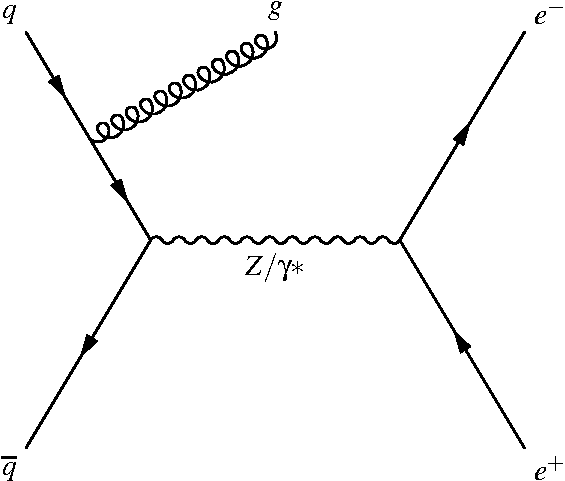
\includegraphics[width=\linewidth]{figures/feyn_qqbar_to_zg.pdf}
        \caption{}
        \label{fig:feyn_qqbar_to_zg}
    \end{subfigure}%
    \begin{subfigure}[b]{\SideBySidePlotWidth}
        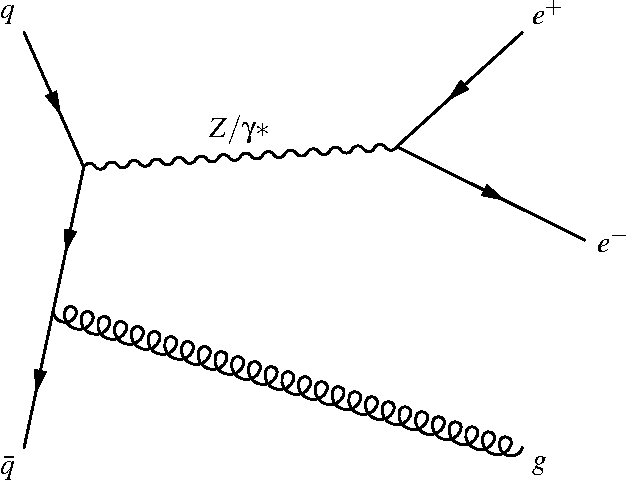
\includegraphics[width=\linewidth]{figures/feyn_qbarq_to_zg.pdf}
        \caption{}
        \label{fig:feyn_qbarq_to_zg}
    \end{subfigure}
    \begin{subfigure}[b]{\SideBySidePlotWidth}
        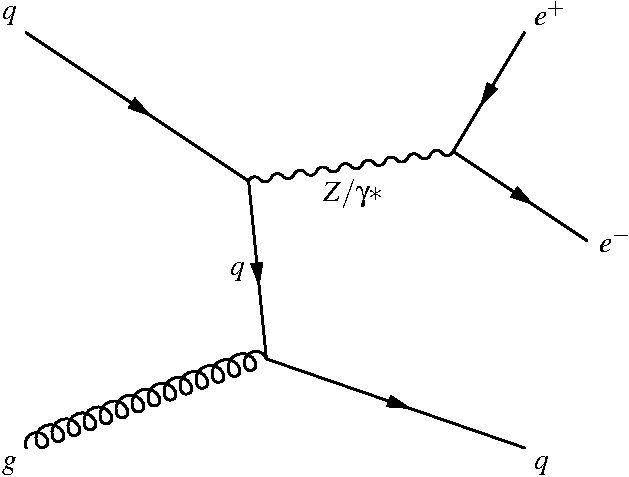
\includegraphics[width=\linewidth]{figures/feyn_qg_to_zq.pdf}
        \caption{}
        \label{fig:feyn_qg_to_zq}
    \end{subfigure}%
    \begin{subfigure}[b]{\SideBySidePlotWidth}
        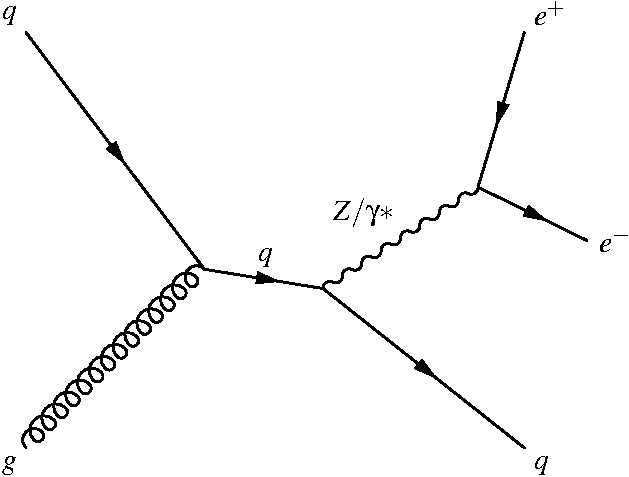
\includegraphics[width=\linewidth]{figures/feyn_qg_to_q_to_zq.pdf}
        \caption{}
        \label{fig:feyn_qg_to_q_to_zq}
    \end{subfigure}
    \caption[
        Higher order in \alphastrong \Ztoee Feynman diagrams.
    ]{
        Higher order in \alphastrong \Ztoee Feynman diagrams. Figures~(a) and
        (b) are ISR where one of the incoming quarks radiates a gluon. In
        \FIGS~(c) and (d) the quark radiates a \Z either before or after
        interacting with a gluon.
    }
    \label{fig:higher_order_z_diagrams}
\end{figure}
